\documentclass{acmsiggraph}               % final

%% These two line bring in essential packages: ``mathptmx'' for Type 1
%% typefaces, and ``graphicx'' for inclusion of EPS figures.


\usepackage{graphicx}
\usepackage{url}
\usepackage{times}
\usepackage{float}



%% Paper title.

\title{Simulate brushed metal surface reflection in homegrown OpenGL render.}

%% Author / Affiliation (single author).

%%\author{Roy G. Biv}
%%\affiliation{Allied Widgets Research\thanks{email:roy.g.biv@aol.com}}

%% Author / Affiliation (multiple authors).

\author{Stefan Eng\thanks{e-mail: atn08sen@student.lth.se}
}
\affiliation{Lund University\\ Sweden}


%% Keywords that describe your work.
\keywords{OpenGL, from-scratch, brushed metal, C}

%%%%%% START OF THE PAPER %%%%%%

\begin{document}

\ifpdf
  \DeclareGraphicsExtensions{.jpg,.pdf,.mps,.png}
\else
  \DeclareGraphicsExtensions{.eps}
\fi


\maketitle

\begin{abstract}
The main motivation for the project is to get accustomed with the limitations
and possibilities of doing low level cross-platform OpenGL programming from scratch in C. The projects
graphical focus is to simulate a brushed metal surface with semi-realistic
anisotropic light reflections. \\

The final approach uses a texture to simulate the
topographic surface features of the brushed metal in combination with a
standard Phong shading model\cite{wiki_phong}.
Ideally this method would be compared to a more procedural approach in
combination with a slightly more advanced light model like the Blinn-Phong
model\cite{wiki_blinn}. This never happened due to the render backbone
implementation hitting a few problems and taking loger then anticipated.

\end{abstract}


\section{Introduction}

\begin{figure}[!ht]
    \centering
    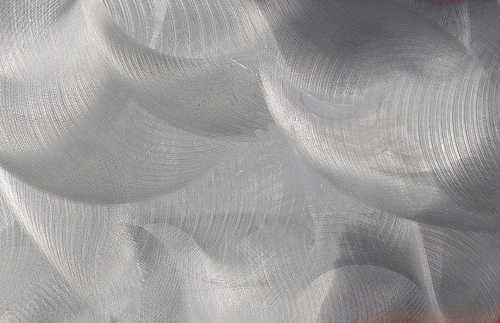
\includegraphics[width=0.7\columnwidth]{brushed.jpg}
    \caption{Photo of brushed metal.}
    \label{brushed_real}
\end{figure}

Brushed metal is a common type of metal texture found on metallic surfaces such
as pots, pans and metallic counter tops. One of the more
recognizable properties of brushed metals is its ability to produce anisotropic
highlights due to the patterned surface area. \\

\begin{figure}[!ht]
    \centering
    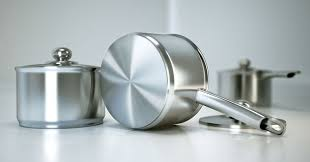
\includegraphics[width=0.7\columnwidth]{highlight.jpg}
    \caption{Example of anisotropic specular highlight.}
    \label{anisotropic_highlight}
\end{figure}

\section{Algorithms}
The algorithm used for simulating bushed metal in this project is \textit{Ward's model of
Anisotropic Reflection}\cite{GregWard}. \\

This model describes reflection in terms of a bidirectional reflectance
distribution function (BRDF), that describes how a light ray from any direction
is reflected into any other direction. Wards BRDF model incorporates two terms;
a diffuse reflectance term and a specular reflectance term.

\subsection{Diffuse term}

The diffuse term is a constant that equals $\frac{\rho_d}{\pi}$ where $\rho_d$
specifies the materials diffuse reflectance. Using the same BRDF
simplifications that are present in the Phong shading model, the diffuse terms
for the color wave lengths Red, Green and Blue can be reduced to pre-defined
material constants.

\subsection{Specular term}

\begin{figure}[!ht]
    \centering
    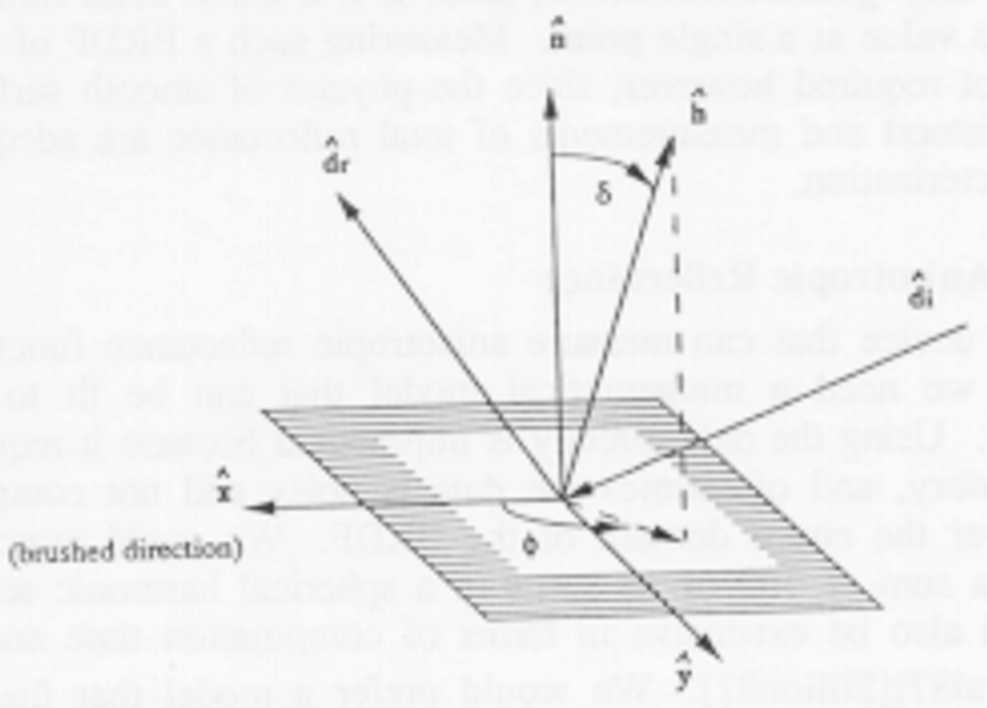
\includegraphics[width=0.7\columnwidth]{figure.png}
    \caption{Fig 5. from Greg Wards paper p. 268}
    \label{figure}
\end{figure}

Using the vector setup above, the following equation can be derived for the
total sum of reflection:
\begin{equation}
  \frac{\rho_d}{pi} + \rho_s \frac{1}{\sqrt{\cos{\theta_i},\cos{\theta_r}}}
  \frac{exp[-\tan^2\delta(\cos^2\phi/\alpha_x^2 +
  \sin^2\phi/\alpha_y^2)]}{4\pi\alpha_x\alpha_y}
\end {equation}

Where $\rho_d$ is the diffuse reflectance, $\rho_s$ is the specular
reflectance, $\alpha_x$ is the standard deviation of the surface slope in the
$\hat{x}$ direction. $\delta$ is the angle between the half vector $\hat{h}$
and the surface normal $\hat{n}$ and $\phi$ is the angle between
$\hat{h}$ projected into the plane and the $\hat{x}$ vector.
\\

By using normal the normalized vectors
\textbf{N},\textbf{V},\textbf{L},\textbf{T},\textbf{B},\textbf{H} for the
normal, view, light, binormal, tangent, and halfway vector, where the halfway vector
is defined as $\textbf{H} = (\textbf{V}+\textbf{L})/|\textbf{V}+\textbf{L}|$,
the earlier formula can then be restated as:
\begin{equation}
  \rho_s \frac{1}{\sqrt{(\textbf{L}\cdot\textbf{N})(\textbf{V}\cdot\textbf{N})}}
  \frac{1}{4\pi\alpha_x\alpha_y} exp (-2\frac{((\textbf{H}\cdot\textbf{T})/\alpha_x)^2)
((\textbf{H}\cdot\textbf{B})/\alpha_y)^2)} {1 + \textbf{H}\cdot\textbf{N}})
  %\sin^2\phi/\alpha_y^2)}{4\pi\alpha_x\alpha_y}
\end {equation}

and since $\rho_s$,$\alpha_x$ and $\alpha_y$ are all constants related to the
diffuse reflectance, the instances outside the exp function can be combined
into the following equation:

\begin{equation}
  k_{specular} \frac{1}{\sqrt{(\textbf{L}\cdot\textbf{N})(\textbf{V}\cdot\textbf{N})}}
  exp (-2\frac{((\textbf{H}\cdot\textbf{T})/\alpha_x)^2)
((\textbf{H}\cdot\textbf{B})/\alpha_y)^2)} {1 + \textbf{H}\cdot\textbf{N}})
  %\sin^2\phi/\alpha_y^2)}{4\pi\alpha_x\alpha_y}
\end {equation}

\section{Implementation}

When implementing the resulting equation in a shader it's important to remember
that the result has to be multiplied with $max(\textbf{L}\cdot\textbf{N},0)$ for
opaque materials to avoid seeing the highlights from the wrong side.
\subsection{Textures}
\begin{figure}[!ht]
    \centering
    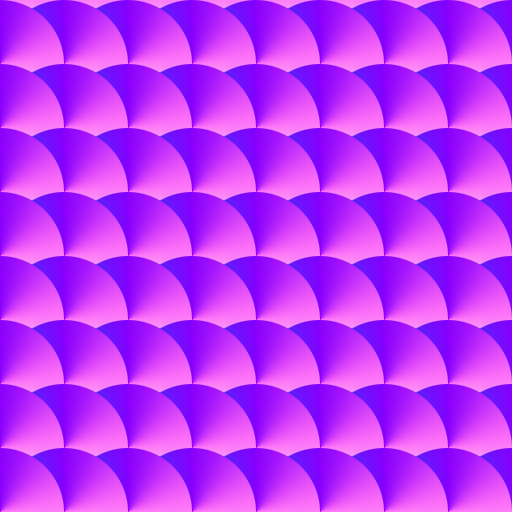
\includegraphics[width=0.5\columnwidth]{aniso_mul.jpg}
    \caption{Tangent-map for several anisotropic patches.}
    \label{figure}
\end{figure}
\begin{figure}[!ht]
    \centering
    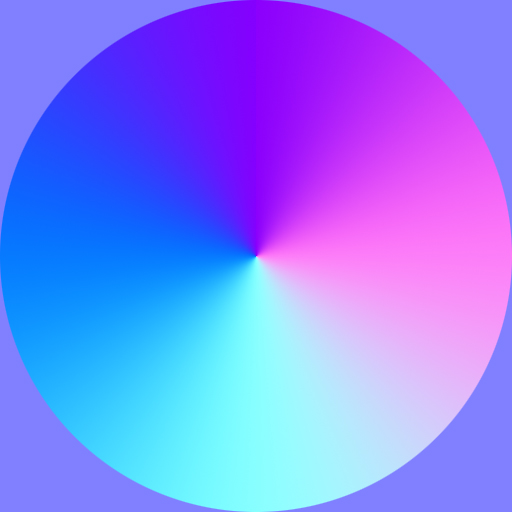
\includegraphics[width=0.5\columnwidth]{aniso_sin.jpg}
    \caption{Tangent-map for single larger anisotropic patch.}
    \label{figure}
\end{figure}
Since the model-data used in this project does not contain any tangents they
are supplied to the shader by sampling the colorvalues from the textures displayed
above. Fitting a combinations of these patterns to the model and using the textures rgb values as
input for the \textbf{T} vector, the equation from earlier is implemented
almost verbatim. The difference being replacing the first term with
$sqrt(max(0, (\textbf{N}\cdot\textbf{L})(\textbf{N}\cdot\textbf{V})))$.
\begin{figure}[H]
    \centering
    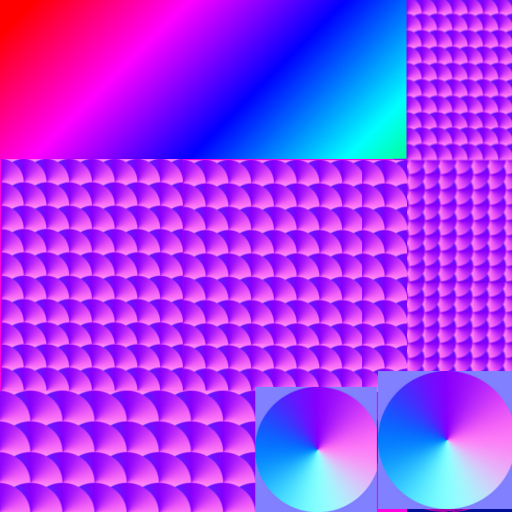
\includegraphics[width=0.5\columnwidth]{anisotropic_direction.jpg}
    \caption{Creating a texture for the coffeepot from patterns.}
    \label{figure}
\end{figure}
\section{Result}

Applying everything mentioned above to the coffeepots in the scene results in
the following effect.

\begin{figure}[H]
    \centering
    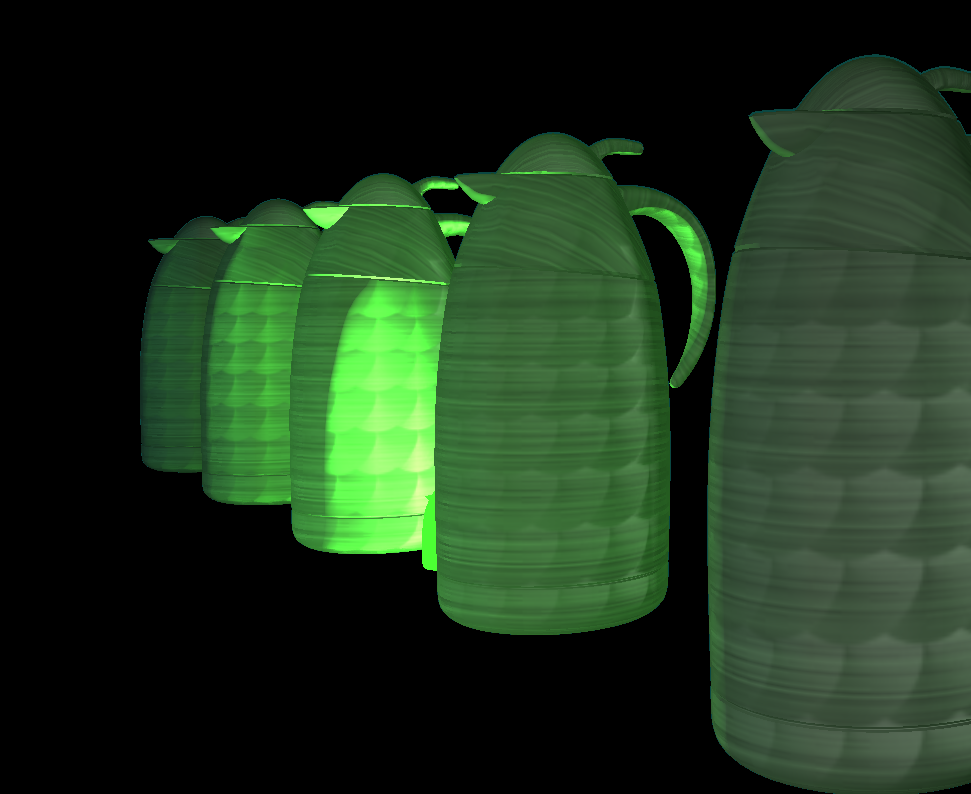
\includegraphics[width=0.7\columnwidth]{result.png}
    \caption{Result of applying shader on coffeepots.}
    \label{figure}
\end{figure}

\section{Conclusion}

The texture-based approach results in a fairly convincing approximation of the
anisotropic reflections. Extra visual enhancements would include bumpmapping on
the brushed base texture as well as environmental cubemapping and lightning. \\

Another conclusion is that writing OpenGL and program-code from scratch in C is super fun and
rewarding, but it takes time.

\bibliographystyle{acmsiggraph}
\bibliography{project}
\end{document}
